\section{pingpong.c}

\subsection{Tổng quan}
\texttt{pingpong.c} minh họa cơ chế giao tiếp liên tiến trình
(\textit{Inter-Process Communication} -- IPC) và đồng bộ giữa tiến trình
cha và tiến trình con trong xv6 \cite{xv6book,mitxv6util2024}.
Chương trình thực hiện một lượt trao đổi dữ liệu (\textit{ping-pong}):
cha gửi một byte cho con, con nhận rồi gửi lại một byte phản hồi cho cha.

Trong xv6, mỗi pipe là một kênh truyền dữ liệu một chiều dưới dạng
luồng byte \cite{xv6book,xv6pipe}. Vì vậy, chương trình sử dụng hai pipe
độc lập để truyền dữ liệu theo hai hướng:
\code{parent\_to\_child} (cha ghi, con đọc) và
\code{child\_to\_parent} (con ghi, cha đọc).

\begin{figure}[H]
    \centering
    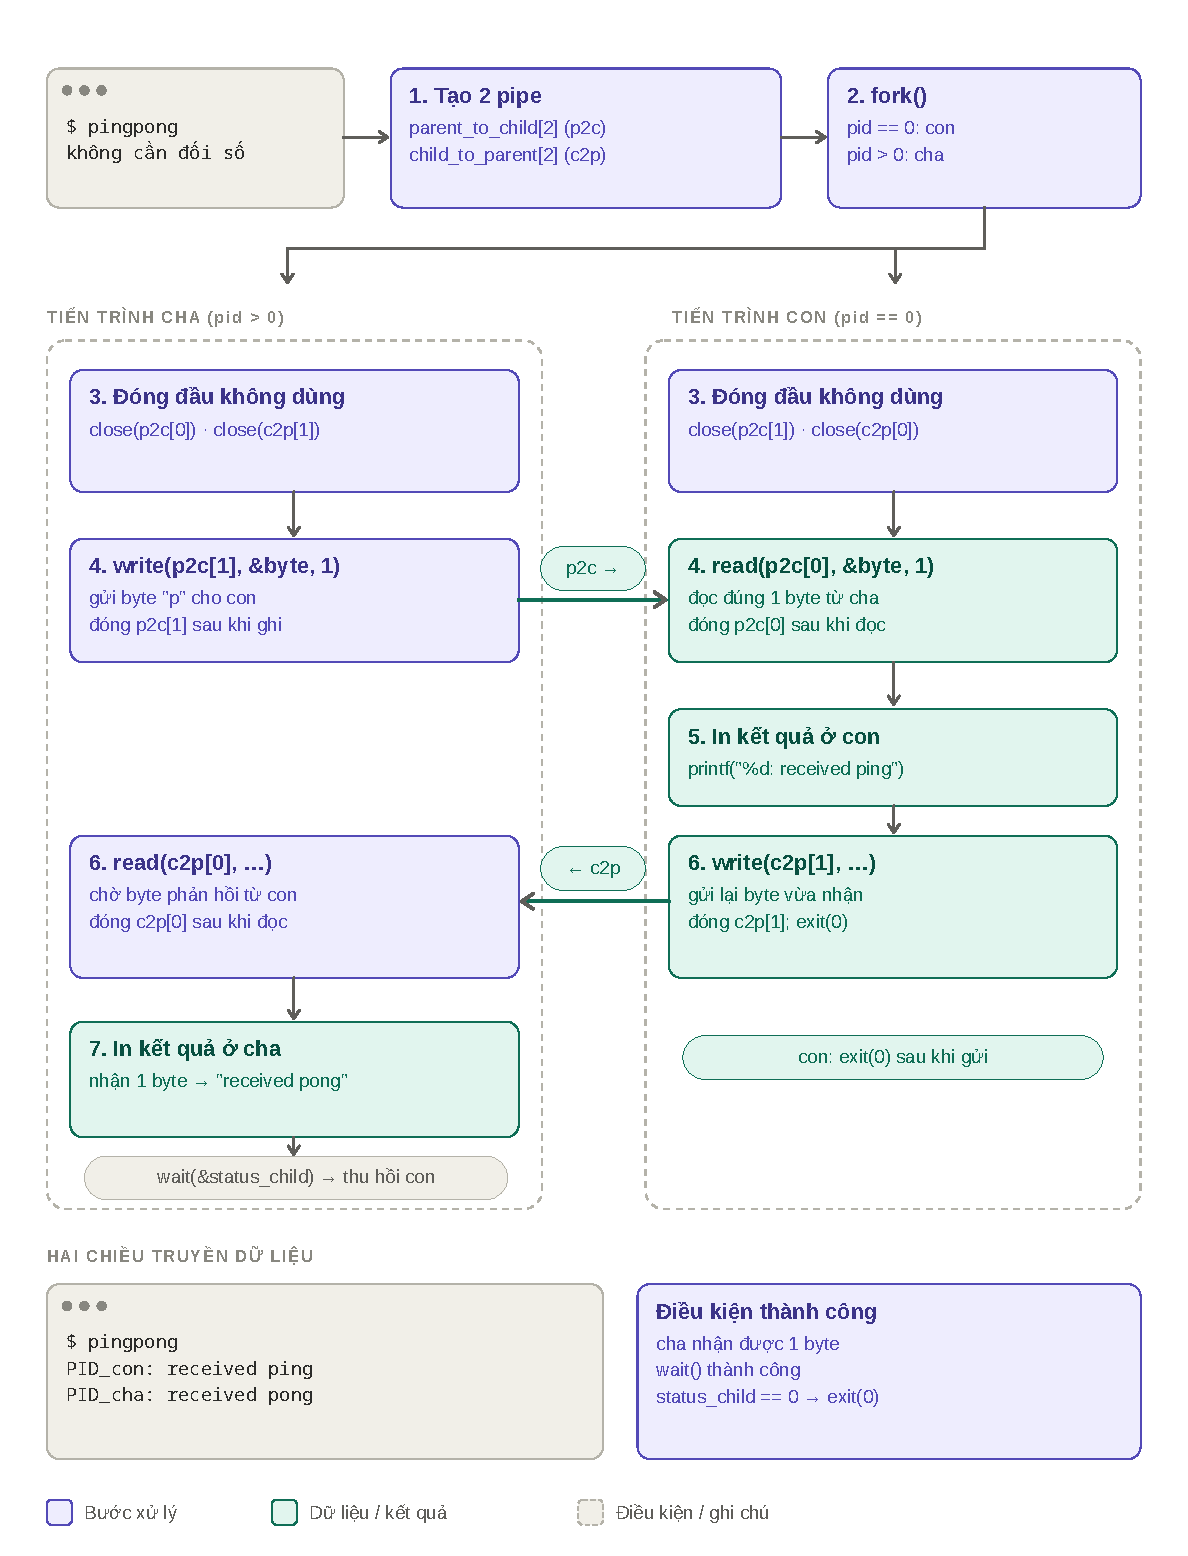
\includegraphics[width=0.47\textwidth]{images/pingpong_workflow.pdf}
    \caption{Sơ đồ giao tiếp IPC qua hai pipe và đồng bộ cha -- con
    trong \texttt{pingpong.c}}
    \label{fig:pingpong_workflow}
\end{figure}

\noindent Luồng thực thi gồm các giai đoạn:
\begin{itemize}[noitemsep, topsep=2pt]
    \item \textbf{Khởi tạo kênh truyền:}
    Tạo hai pipe, sau đó gọi \code{fork()} để sinh tiến trình con.
    Hai tiến trình đóng những đầu pipe không sử dụng nhằm tránh giữ
    file descriptor (FD) không cần thiết (Bảng \ref{tab:pingpong_pipes}).

    \item \textbf{Trao đổi dữ liệu:}
    Cha gửi byte \code{'p'} qua pipe \code{parent\_to\_child[1]}.
    Con đọc dữ liệu từ \code{parent\_to\_child[0]}, in dòng
    \texttt{<pid>: received ping}, rồi gửi lại một byte qua
    \code{child\_to\_parent[1]}.
    Cha nhận phản hồi từ pipe \code{child\_to\_parent[0]} và in
    \texttt{<pid>: received pong}.

    \item \textbf{Thu hồi tài nguyên:}
    Hai tiến trình đóng các đầu pipe còn sử dụng sau khi hoàn tất I/O.
    Cha gọi \code{wait(\&status\_child)} để chờ và thu hồi tiến trình con,
    đồng thời kiểm tra kết quả trước khi kết thúc.
\end{itemize}

\begin{table}[H]
    \centering
    \small
    \begin{tabularx}{0.85\textwidth}{lXX}
        \toprule
        Pipe & Cha giữ & Con giữ \\
        \midrule
        \texttt{parent\_to\_child} & Đầu ghi \texttt{[1]} & Đầu đọc \texttt{[0]} \\
        \texttt{child\_to\_parent} & Đầu đọc \texttt{[0]} & Đầu ghi \texttt{[1]} \\
        \bottomrule
    \end{tabularx}
    \caption{Các đầu pipe mỗi tiến trình cần giữ sau \code{fork()}}
    \label{tab:pingpong_pipes}
\end{table}

\subsection{Khó khăn và Thử thách}
Trong quá trình hiện thực cơ chế IPC của xv6, nhóm tập trung xử lý
các vấn đề về file descriptor, thứ tự trao đổi dữ liệu và quản lý
vòng đời tiến trình \cite{xv6book,remzi2018ostep}.

\begin{enumerate}[noitemsep, topsep=2pt]
    \item \textbf{Đóng đầu ghi pipe và kiểm soát điều kiện EOF:}
    Khi pipe rỗng nhưng vẫn còn đầu ghi được mở, \code{read()} sẽ chờ
    dữ liệu mới; lệnh chỉ trả về 0 (EOF) khi toàn bộ các đầu ghi đã đóng
    \cite{xv6book,xv6pipe}.
    Tuy nhiên, với thao tác đọc đúng một byte của chương trình, việc giữ
    đầu ghi thừa không tự động gây deadlock nếu byte dữ liệu đã đến.
    Nguy cơ chờ vô hạn xuất hiện khi chương trình tiếp tục đọc trên pipe
    rỗng để đợi EOF mà vẫn còn một bản sao đầu ghi được giữ mở.\\
    \textit{Giải pháp:}
    Sau \code{fork()}, con đóng \code{parent\_to\_child[1]} và
    \code{child\_to\_parent[0]}; cha đóng \code{parent\_to\_child[0]}
    và \code{child\_to\_parent[1]}.
    Mỗi tiến trình tiếp tục đóng đầu ghi sau khi gửi xong và đóng đầu
    đọc sau khi nhận xong.

    \item \textbf{Đảm bảo thứ tự hiển thị giữa hai tiến trình:}
    Sau \code{fork()}, lịch chạy của cha và con không cố định.
    Nếu cho hai tiến trình in kết quả độc lập, thứ tự có thể thay đổi.\\
    \textit{Giải pháp:}
    Sử dụng cơ chế \textit{blocking I/O} của pipe để đồng bộ:
    con chỉ in \texttt{received ping} sau khi nhận byte từ cha,
    rồi mới gửi phản hồi; cha chỉ in \texttt{received pong} sau khi
    đọc được phản hồi từ con.
    Vì vậy, thứ tự hai thông báo được xác lập thông qua chính luồng
    trao đổi dữ liệu, không cần cơ chế khóa bổ sung
    \cite{xv6book,mitxv6util2024}.

    \item \textbf{Xử lý lỗi khởi tạo và thu hồi tiến trình:}
    \code{pipe()} và \code{fork()} có thể thất bại khi tài nguyên hệ thống
    không đủ. Trong xv6-riscv, \code{NPROC = 64} giới hạn số tiến trình,
    còn \code{NOFILE = 16} giới hạn số FD mở trên mỗi tiến trình
    \cite{xv6param}.
    Tiến trình con đã thoát sẽ ở trạng thái zombie cho đến khi được
    thu hồi. Nếu cha thoát trước, xv6 chuyển tiến trình con còn lại
    cho \code{init}; đồng thời, \code{exit()} tự đóng các FD đang mở
    \cite{xv6book,xv6proc}.\\
    \textit{Giải pháp:}
    Kiểm tra kết quả mỗi lời gọi \code{pipe()} và \code{fork()}.
    Nếu khởi tạo thất bại, chương trình đóng các FD đã tạo rồi thoát
    với mã lỗi. Trong luồng thành công, cha gọi \code{wait()} để thu hồi
    con, tránh để zombie tồn tại trong thời gian cha còn hoạt động.
\end{enumerate}

\section{cp.c}

\subsection{Tổng quan}
\texttt{cp.c} hiện thực chức năng sao chép nội dung của một tệp thông
thường sang một đường dẫn đích trong xv6, tham khảo tiện ích
\texttt{cp} của POSIX \cite{posix2018cp}.
Phiên bản này hỗ trợ cú pháp cơ bản \code{cp src dst}, không nhằm
triển khai toàn bộ tùy chọn và trường hợp sử dụng của POSIX \texttt{cp}.

Trong xv6, thông tin tệp được quản lý bằng inode; cặp giá trị
\texttt{(dev, ino)} giúp xác định hai đường dẫn có đang tham chiếu đến
cùng một inode hay không \cite{xv6book}.
Chương trình đọc dữ liệu từ tệp nguồn được mở bằng \code{O\_RDONLY}
và ghi sang tệp đích bằng tổ hợp cờ
\code{O\_WRONLY} $|$ \code{O\_CREATE} $|$ \code{O\_TRUNC},
thông qua bộ đệm có kích thước cố định.

\begin{figure}[H]
    \centering
    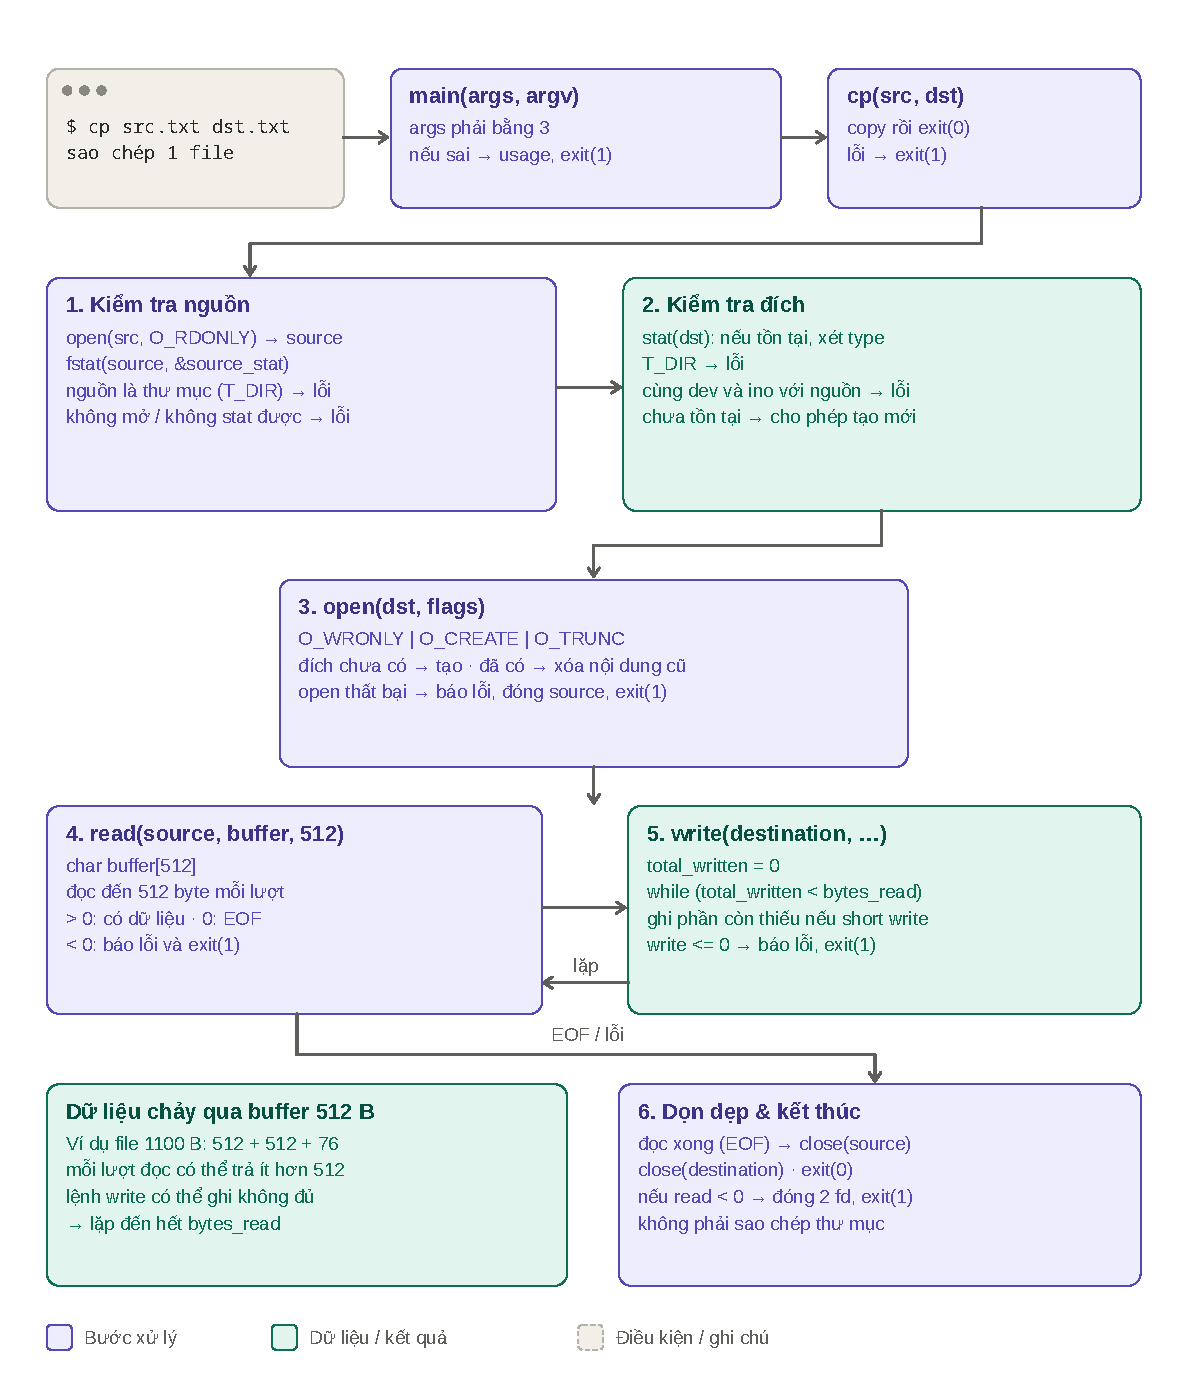
\includegraphics[width=0.70\textwidth]{images/cp_workflow.pdf}
    \caption{Sơ đồ kiểm tra inode và sao chép dữ liệu theo khối
    trong \texttt{cp.c}}
    \label{fig:cp_workflow}
\end{figure}

\noindent Luồng thực thi gồm các giai đoạn:
\begin{itemize}[noitemsep, topsep=2pt]
    \item \textbf{Kiểm tra đối số và tệp:}
    Yêu cầu đúng hai đối số đường dẫn (\code{argc == 3}), mở tệp nguồn
    bằng \code{O\_RDONLY} và dùng \code{fstat()} để từ chối thư mục.
    Nếu đích đã tồn tại, dùng \code{stat()} kiểm tra kiểu tệp và so sánh
    cặp \code{dev}, \code{ino} nhằm phát hiện trường hợp trùng tệp.

    \item \textbf{Mở đích và chuẩn bị bộ đệm:}
    Sau khi kiểm tra, mở tệp đích với tổ hợp các cờ
    \code{O\_WRONLY} $|$ \code{O\_CREATE} $|$ \code{O\_TRUNC}.
    Sử dụng bộ đệm \code{buffer[512]} để truyền dữ liệu theo từng khối.

    \item \textbf{Sao chép dữ liệu:}
    Lặp lại việc \code{read()} tối đa 512 byte từ nguồn, rồi ghi dữ liệu
    đã đọc sang đích. Vòng lặp ghi kiểm tra số byte được ghi và tiếp
    tục nếu còn dữ liệu chưa ghi hết. Khi \code{read()} trả về 0 (EOF),
    chương trình đóng các FD và kết thúc thành công; nếu I/O trả về
    lỗi, chương trình chuyển sang nhánh xử lý lỗi.
\end{itemize}

\subsection{Khó khăn và Thử thách}
Trong quá trình xây dựng thao tác sao chép tệp trên xv6, nhóm
chú trọng việc tránh ghi đè nhầm tệp nguồn, kiểm tra kết quả I/O
và dọn dẹp tài nguyên \cite{xv6book}.

\begin{enumerate}[noitemsep, topsep=2pt]
    \item \textbf{Ngăn việc ghi đè vào chính tệp nguồn:}
    Nếu nguồn và đích trỏ đến cùng một inode, thao tác mở đích
    với \code{O\_TRUNC} sẽ cắt kích thước của tệp thường về 0,
    khiến dữ liệu nguồn bị mất trước khi sao chép
    \cite{xv6sysfile}.\\
    \textit{Giải pháp:}
    Trước khi mở đích, chương trình dùng \code{stat()} để đối chiếu:
    \code{source\_stat.dev} $==$ \code{destination\_stat.dev} cùng với
    \code{source\_stat.ino} $==$ \code{destination\_stat.ino}.
    Nếu cả hai điều kiện trên đều thỏa mãn, chương trình thông báo lỗi và đóng
    FD nguồn mà không thực hiện \code{O\_TRUNC}.

    \item \textbf{Kiểm tra kết quả ghi dữ liệu:}
    Trong giao diện I/O kiểu Unix, mã trả về của \code{write()} cần
    được kiểm tra thay vì giả định mọi lần ghi đều hoàn tất.
    Riêng trên xv6, đường ghi của tệp thông thường xử lý nhiều khối
    trong kernel và thường trả về đủ số byte yêu cầu hoặc mã lỗi
    \cite{xv6file}.\\
    \textit{Giải pháp:}
    Dùng biến \code{total\_written} để theo dõi lượng dữ liệu đã ghi.
    Nếu \code{write()} trả về số byte dương nhỏ hơn số byte cần ghi,
    chương trình tiếp tục ghi tiếp từ vị trí
    \code{buffer} $+$ \code{total\_written}; nếu trả về giá trị không dương,
    chương trình xử lý như lỗi ghi.

    \item \textbf{Từ chối sao chép thư mục và dọn dẹp FD:}
    Thư mục trong xv6 chứa dữ liệu cấu trúc hệ thống tệp.
    Việc sao chép thô các byte này sang tệp thường không tương đương
    với sao chép cây thư mục \cite{xv6book}.\\
    \textit{Giải pháp:}
    Dùng \code{fstat()} hoặc \code{stat()} để từ chối nguồn hoặc đích
    có kiểu \code{T\_DIR}. Khi \code{open()}, \code{read()} hoặc
    \code{write()} thất bại, chương trình đóng các FD đã mở và trả về
    mã lỗi, thay vì tiếp tục với dữ liệu chưa được sao chép đầy đủ.
\end{enumerate}